\documentclass[aspectratio=43,17pt]{beamer} % or 14 or 17 or 20

\usepackage{tikz,pgf,lmodern,textpos,hyperref,graphicx,booktabs,appendixnumberbeamer,cleveref,fancybox,multicol}
% \usepackage[fontsize=18]{pdfpcnotes}
\usepackage{pgfcalendar,svg,subfiles,chronosys,cancel,xcolor,color,nth,datenumber,xparse,fp,stackengine,makecell}
\usepackage{amsmath}
\usepackage{centernot}
\usetikzlibrary{positioning}
\usepackage[outline]{contour}
\usepackage[citestyle=authoryear-comp,backend=bibtex]{biblatex}
\usepackage[export]{adjustbox}
\usepackage[en-US]{datetime2}
\usepackage[normalem]{ulem}
\bibliography{references}
\usetheme[numbering=none]{metropolis}

% \bibliography{references}

%!TEX Root = ./presentation.tex

\definecolor{Blue}{HTML}{00548f}
\definecolor{Cardinal Red}{HTML}{8c1515}
\definecolor{White}{HTML}{ffffff}
\definecolor{Cool Grey}{HTML}{4d4f53}
\definecolor{Black}{HTML}{2e2d29}
\definecolor{Bright Red}{HTML}{B1040E}
\definecolor{Dark Red}{HTML}{820000}
\definecolor{Chocolate}{HTML}{2F2424}
\definecolor{Stone}{HTML}{544948}
\definecolor{Fog}{HTML}{F4F4F4}
\definecolor{Light Sandstone}{HTML}{F9F6EF}
\definecolor{Sandstone}{HTML}{d2c295}
\definecolor{Warm Grey}{HTML}{3f3c30}
\definecolor{Beige}{HTML}{9d9573}
\definecolor{Light Sage}{HTML}{c7d1c5}
\definecolor{Clay}{HTML}{5f574f}
\definecolor{Cloud}{HTML}{dad7cb}
\definecolor{Driftwood}{HTML}{b6b1a9}
\definecolor{Stone}{HTML}{928b81}
\definecolor{Sandhill}{HTML}{b3995d}
\definecolor{Palo Alto}{HTML}{175e54}
\definecolor{Teal}{HTML}{00505c}
\definecolor{Purple}{HTML}{53284f}
\definecolor{Redwood}{HTML}{8d3c1e}
\definecolor{Brown}{HTML}{5e3032}
\definecolor{Sky}{HTML}{0098db}
\definecolor{Lagunita}{HTML}{007c92}
\definecolor{Mint}{HTML}{009b76}
\definecolor{Gold}{HTML}{b26f16}
\definecolor{Sun}{HTML}{eaab00}
\definecolor{Poppy}{HTML}{e98300}

\definecolor{USF Green}{HTML}{00543C}
\definecolor{USF Gold}{HTML}{FDBB30}
\definecolor{USF Grey}{HTML}{919194}
% \definecolor{USF }{HTML}{e98300}


\setbeamercolor{normal text}{fg=Black,bg=White}
\hypersetup{colorlinks,linkcolor=USF Green,urlcolor=USF Green,citecolor=USF Green}
% \setbeamercolor{frametitle}{bg=Cardinal Red, fg=Blue}


\setbeamercolor{palette primary}{bg=Fog, fg=USF Green}
\setbeamercolor{palette secondary}{bg=USF Green, fg=Fog}
\setbeamercolor{frametitle}{bg=Fog,fg=USF Green}

% \setbeamercolor{section title}{fg=Dark Red, bg=Fog}
\setbeamercolor{alerted text}{fg=USF Green}

\newcommand{\soutthick}[1]{%
    \renewcommand{\ULthickness}{2.4pt}%
       \sout{#1}%
    \renewcommand{\ULthickness}{.4pt}% Resetting to ulem default
}


  \setbeamercolor{normal text}{%
    fg=Cool Grey,
    bg=White
  }

\setbeamercolor{palette primary}{fg=Fog, bg=Dark Red}
\setbeamercolor{palette secondary}{bg=Dark Red, bg=Fog}
\setbeamercovered{transparent}
% \setbeamercolor{background canvas}{bg=Fog}
\setbeamercolor{frametitle}{bg=Dark Red,fg=Fog}
\hypersetup{colorlinks,linkcolor=Blue,urlcolor=Blue,citecolor=Blue}
\setbeamercolor{alerted text}{fg=Bright Red}
\setbeamertemplate{caption}{\insertcaption}


\setsansfont[BoldFont={Source Sans Pro Bold},
              Numbers={OldStyle}]{Source Sans Pro}
\setmainfont[BoldFont={Source Serif Pro Semibold},
              Numbers={OldStyle}]{Source Serif Pro}
\setmonofont{Source Code Pro}


\metroset{titleformat=smallcaps,numbering=none}


\newenvironment{mystepwiseitemize}{\begin{itemize}[<+-| alert@+>]}{\end{itemize}}




\title{Data Ethics Lecture 2}
\subtitle{recap {\bfseries Data Collection}\\preview {\bfseries Promises}}
\author[Ali Alkhatib]{{Ali Alkhatib}\\
\href{http://twitter.com/_alialkhatib}{@\_alialkhatib} || \href{mailto:hi@al2.in}{hi@al2.in}}
\date{March 17, 2022}

% \date{\today}


\newcommand{\onlyinsubfile}[1]{#1}
\newcommand{\notinsubfile}[1]{}

\begin{document}
\renewcommand{\onlyinsubfile}[1]{}
\renewcommand{\notinsubfile}[1]{#1}


\begin{frame}
\titlepage
\end{frame}

\begin{frame}[t]\frametitle{Roadmap for today}

\begin{itemize}
    \item Administrivia
    \item Recap Data Collection
    \item Preview Promises
    \item Discuss 1 or 2 promises
    \item Preview readings for 1-2 topics
\end{itemize}

\end{frame}


\begin{frame}{Admin-y things}
  

\begin{itemize}
    \item \strong{Canvas}
    
    {\small everyone should have access now, if that's not the case then let me know!}
    \item \strong{Readings}
    
    {\small More readings available on Canvas as PDFs}
    \item \strong{Reading time check}

    {\small How long did readings take?}
    
    \item \strong{great reflections, everyone}
\end{itemize}

\end{frame}


\section{Data Collection (recap)}

\begin{frame}[t]{consent}
\begin{columns}
\begin{column}{0.4\textwidth}
\only<1-4>{\alert{\strong{legally ambiguous}} data collection}%
\only<5->{legislative \alert{\strong{reforms}}}
\end{column}
\begin{column}{0.6\textwidth}
\only<1>{\includegraphics[width=\textwidth]{figures/consent/CTL.PNG}}
\only<2>{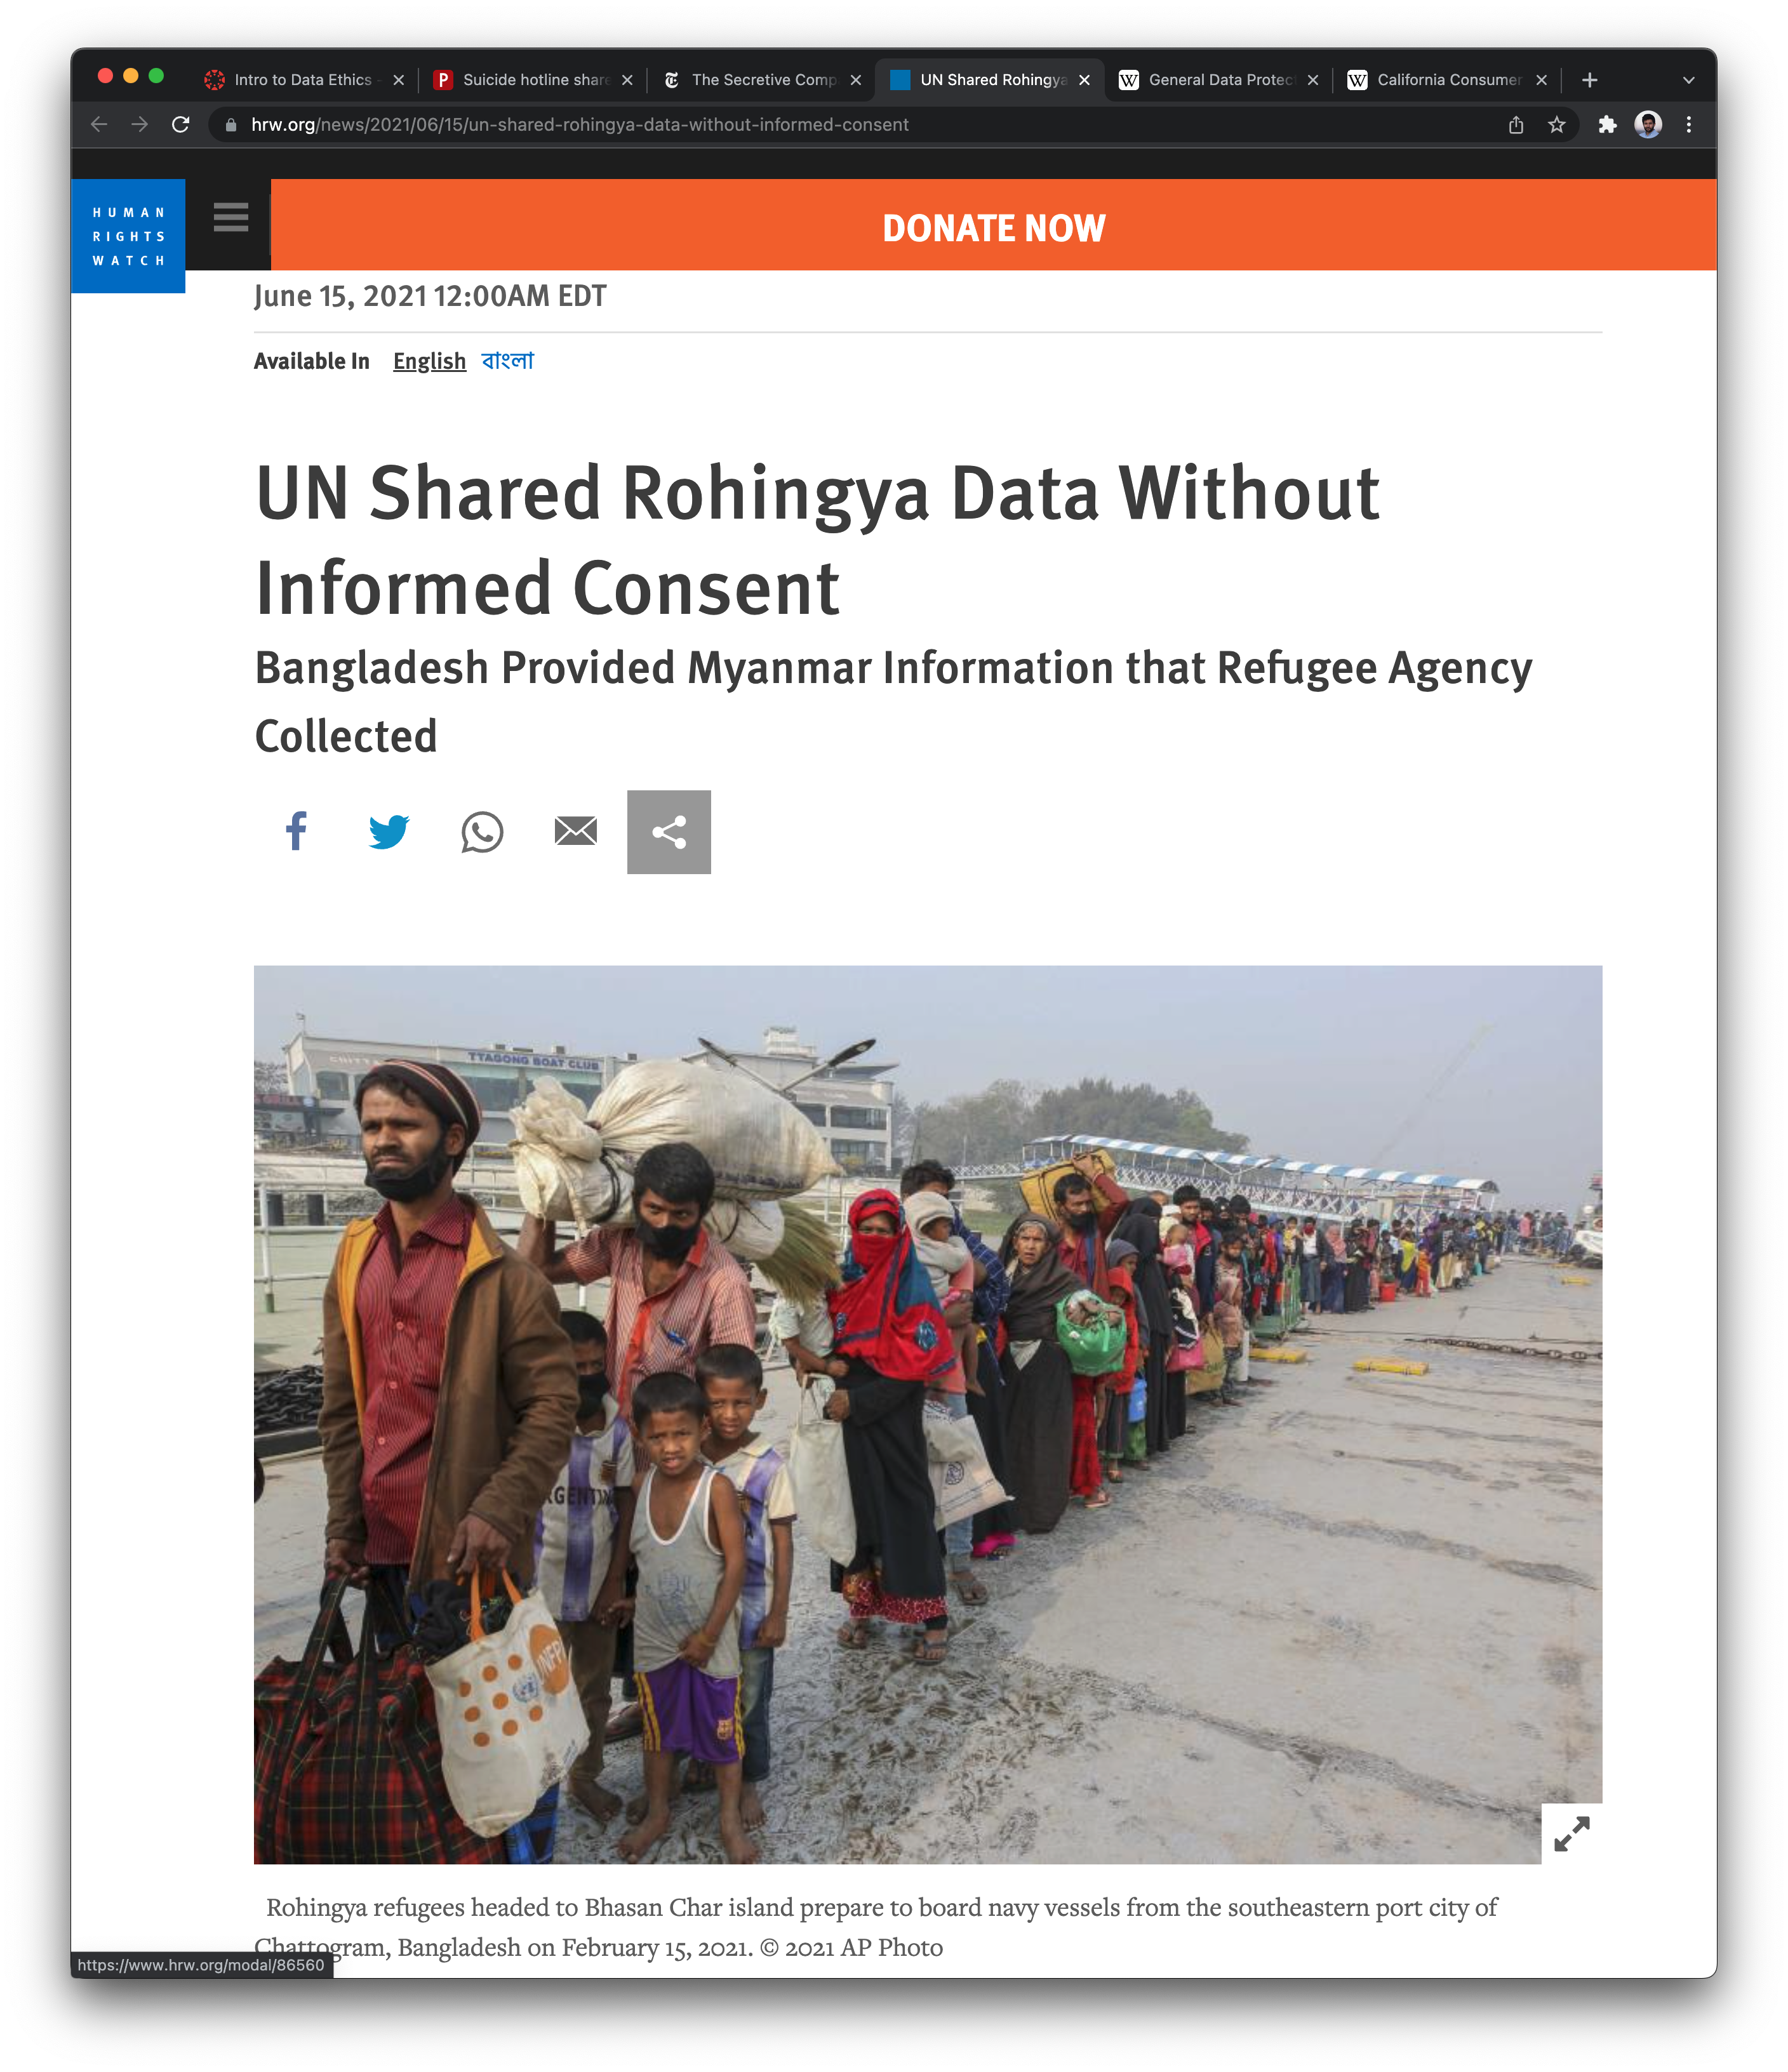
\includegraphics[width=\textwidth]{figures/consent/rohingya.png}}
\only<3>{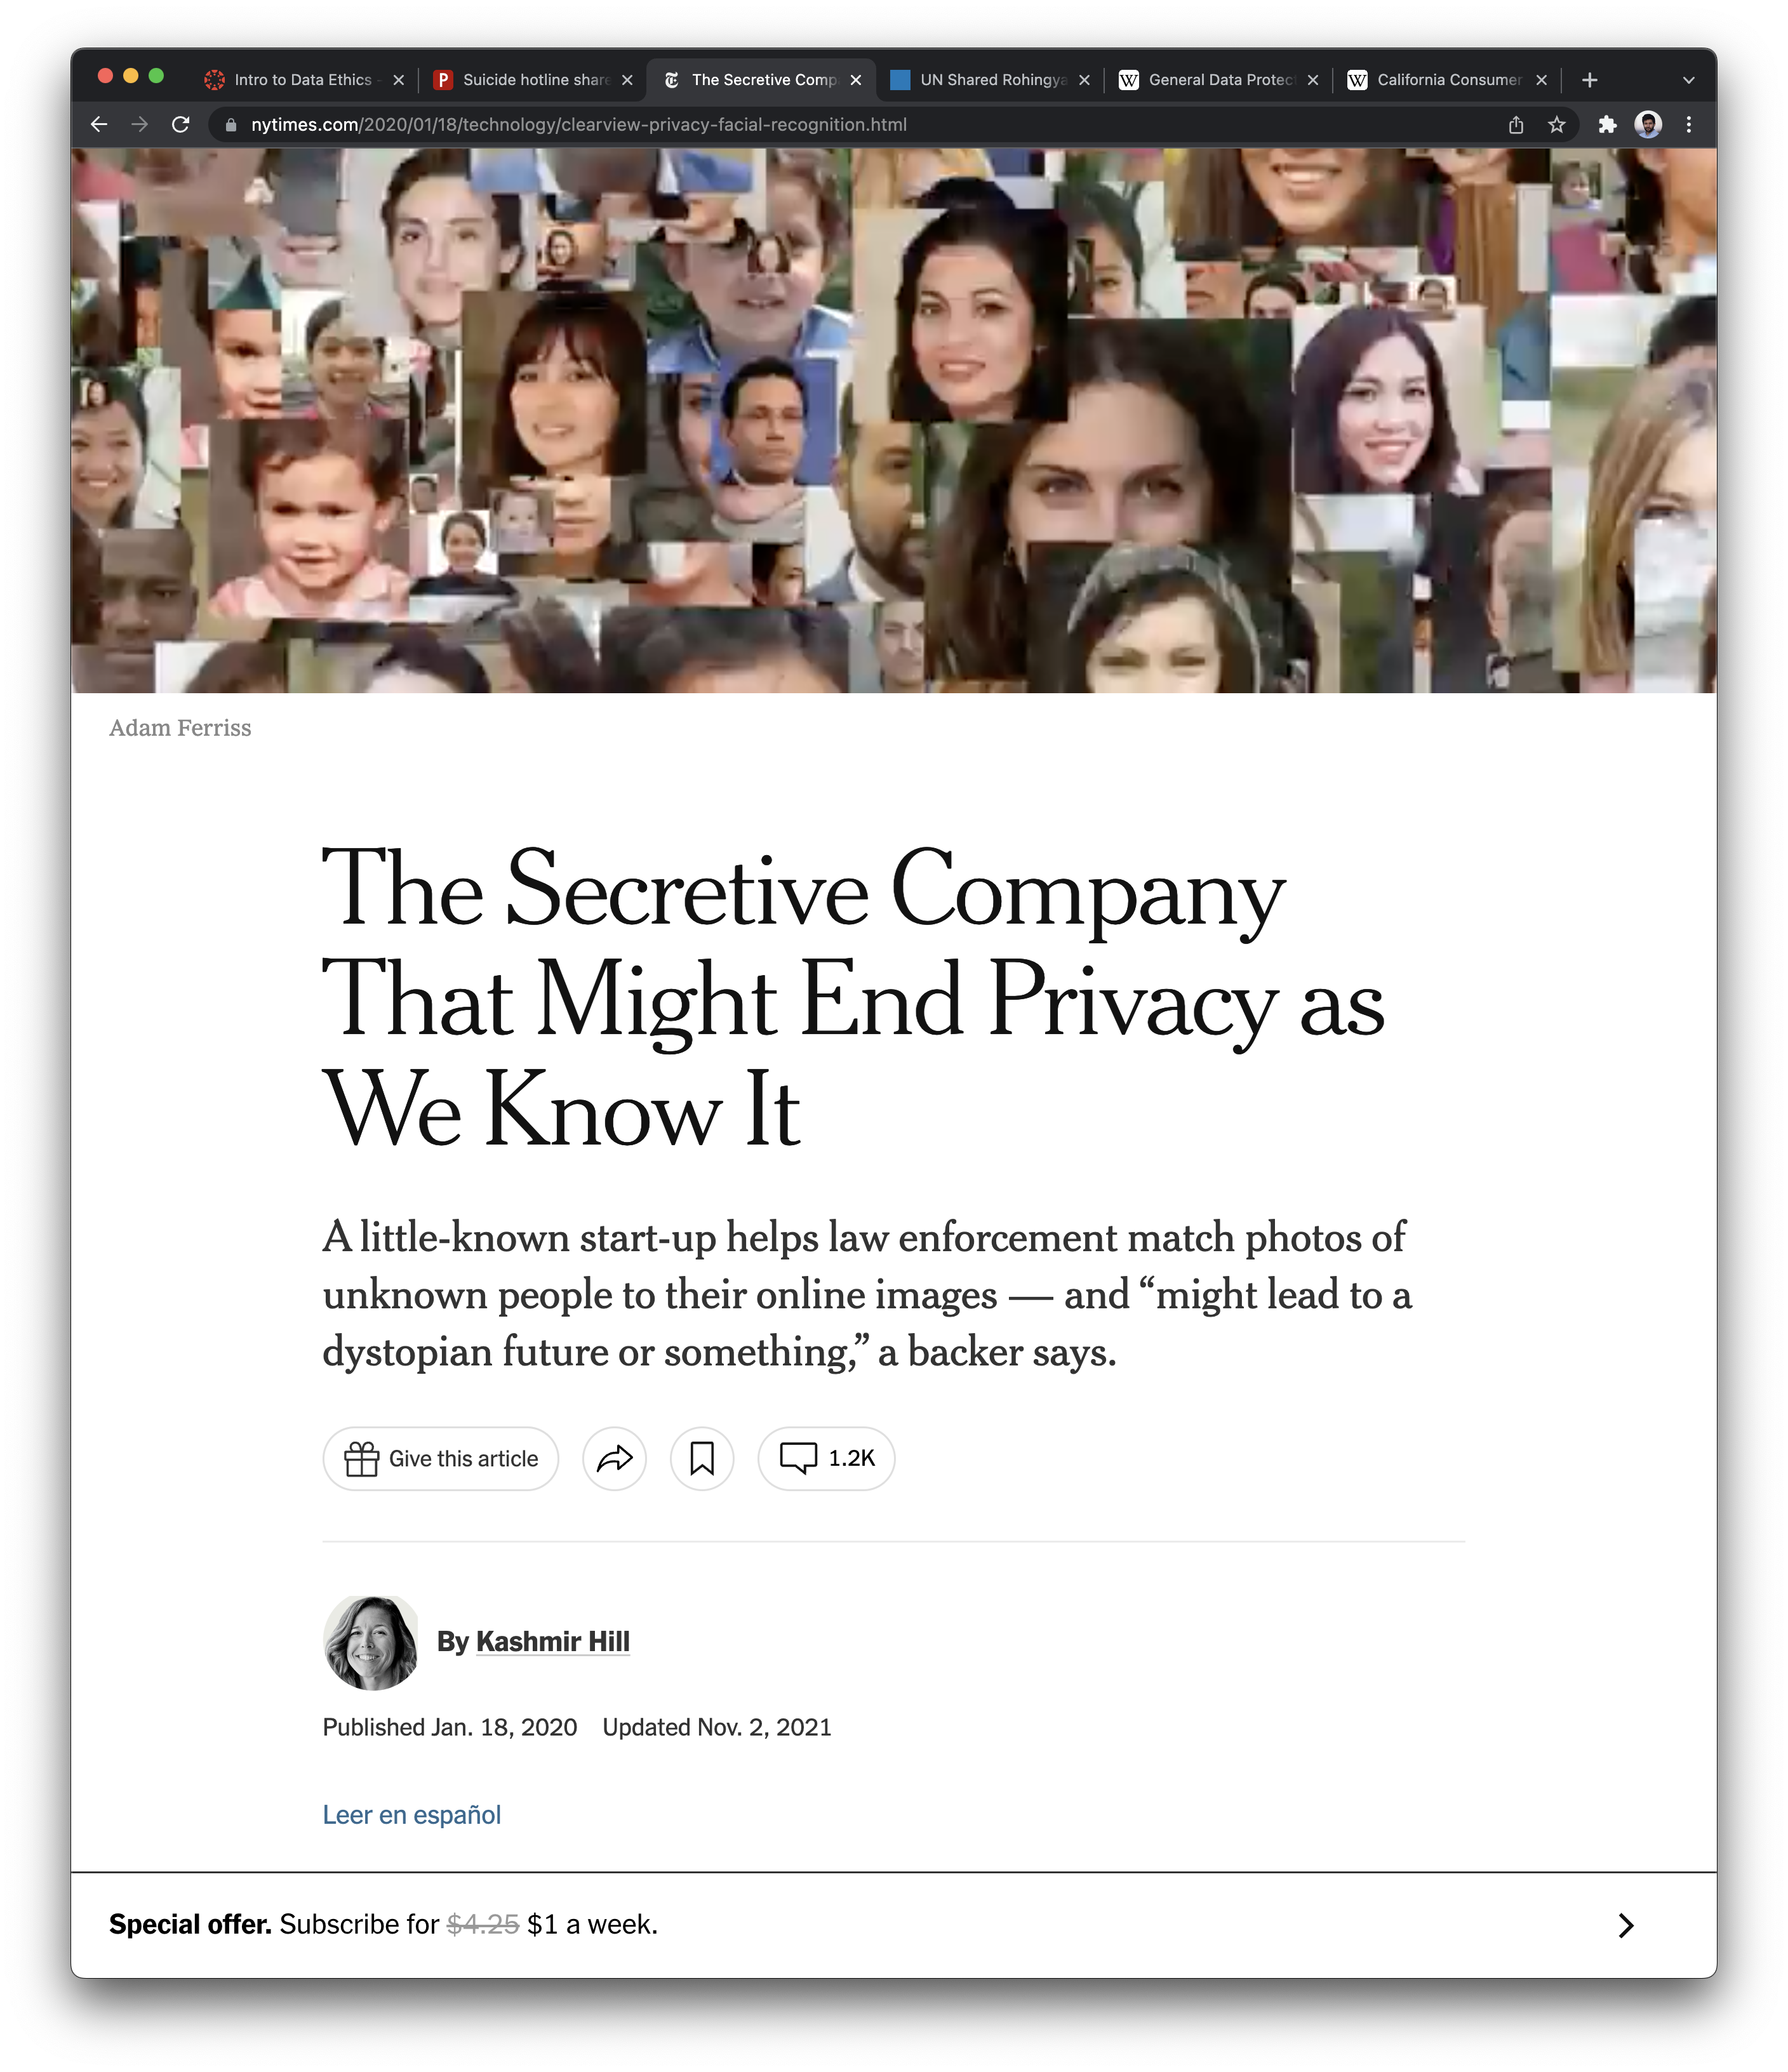
\includegraphics[width=\textwidth]{figures/consent/clearview.png}}
\only<4>{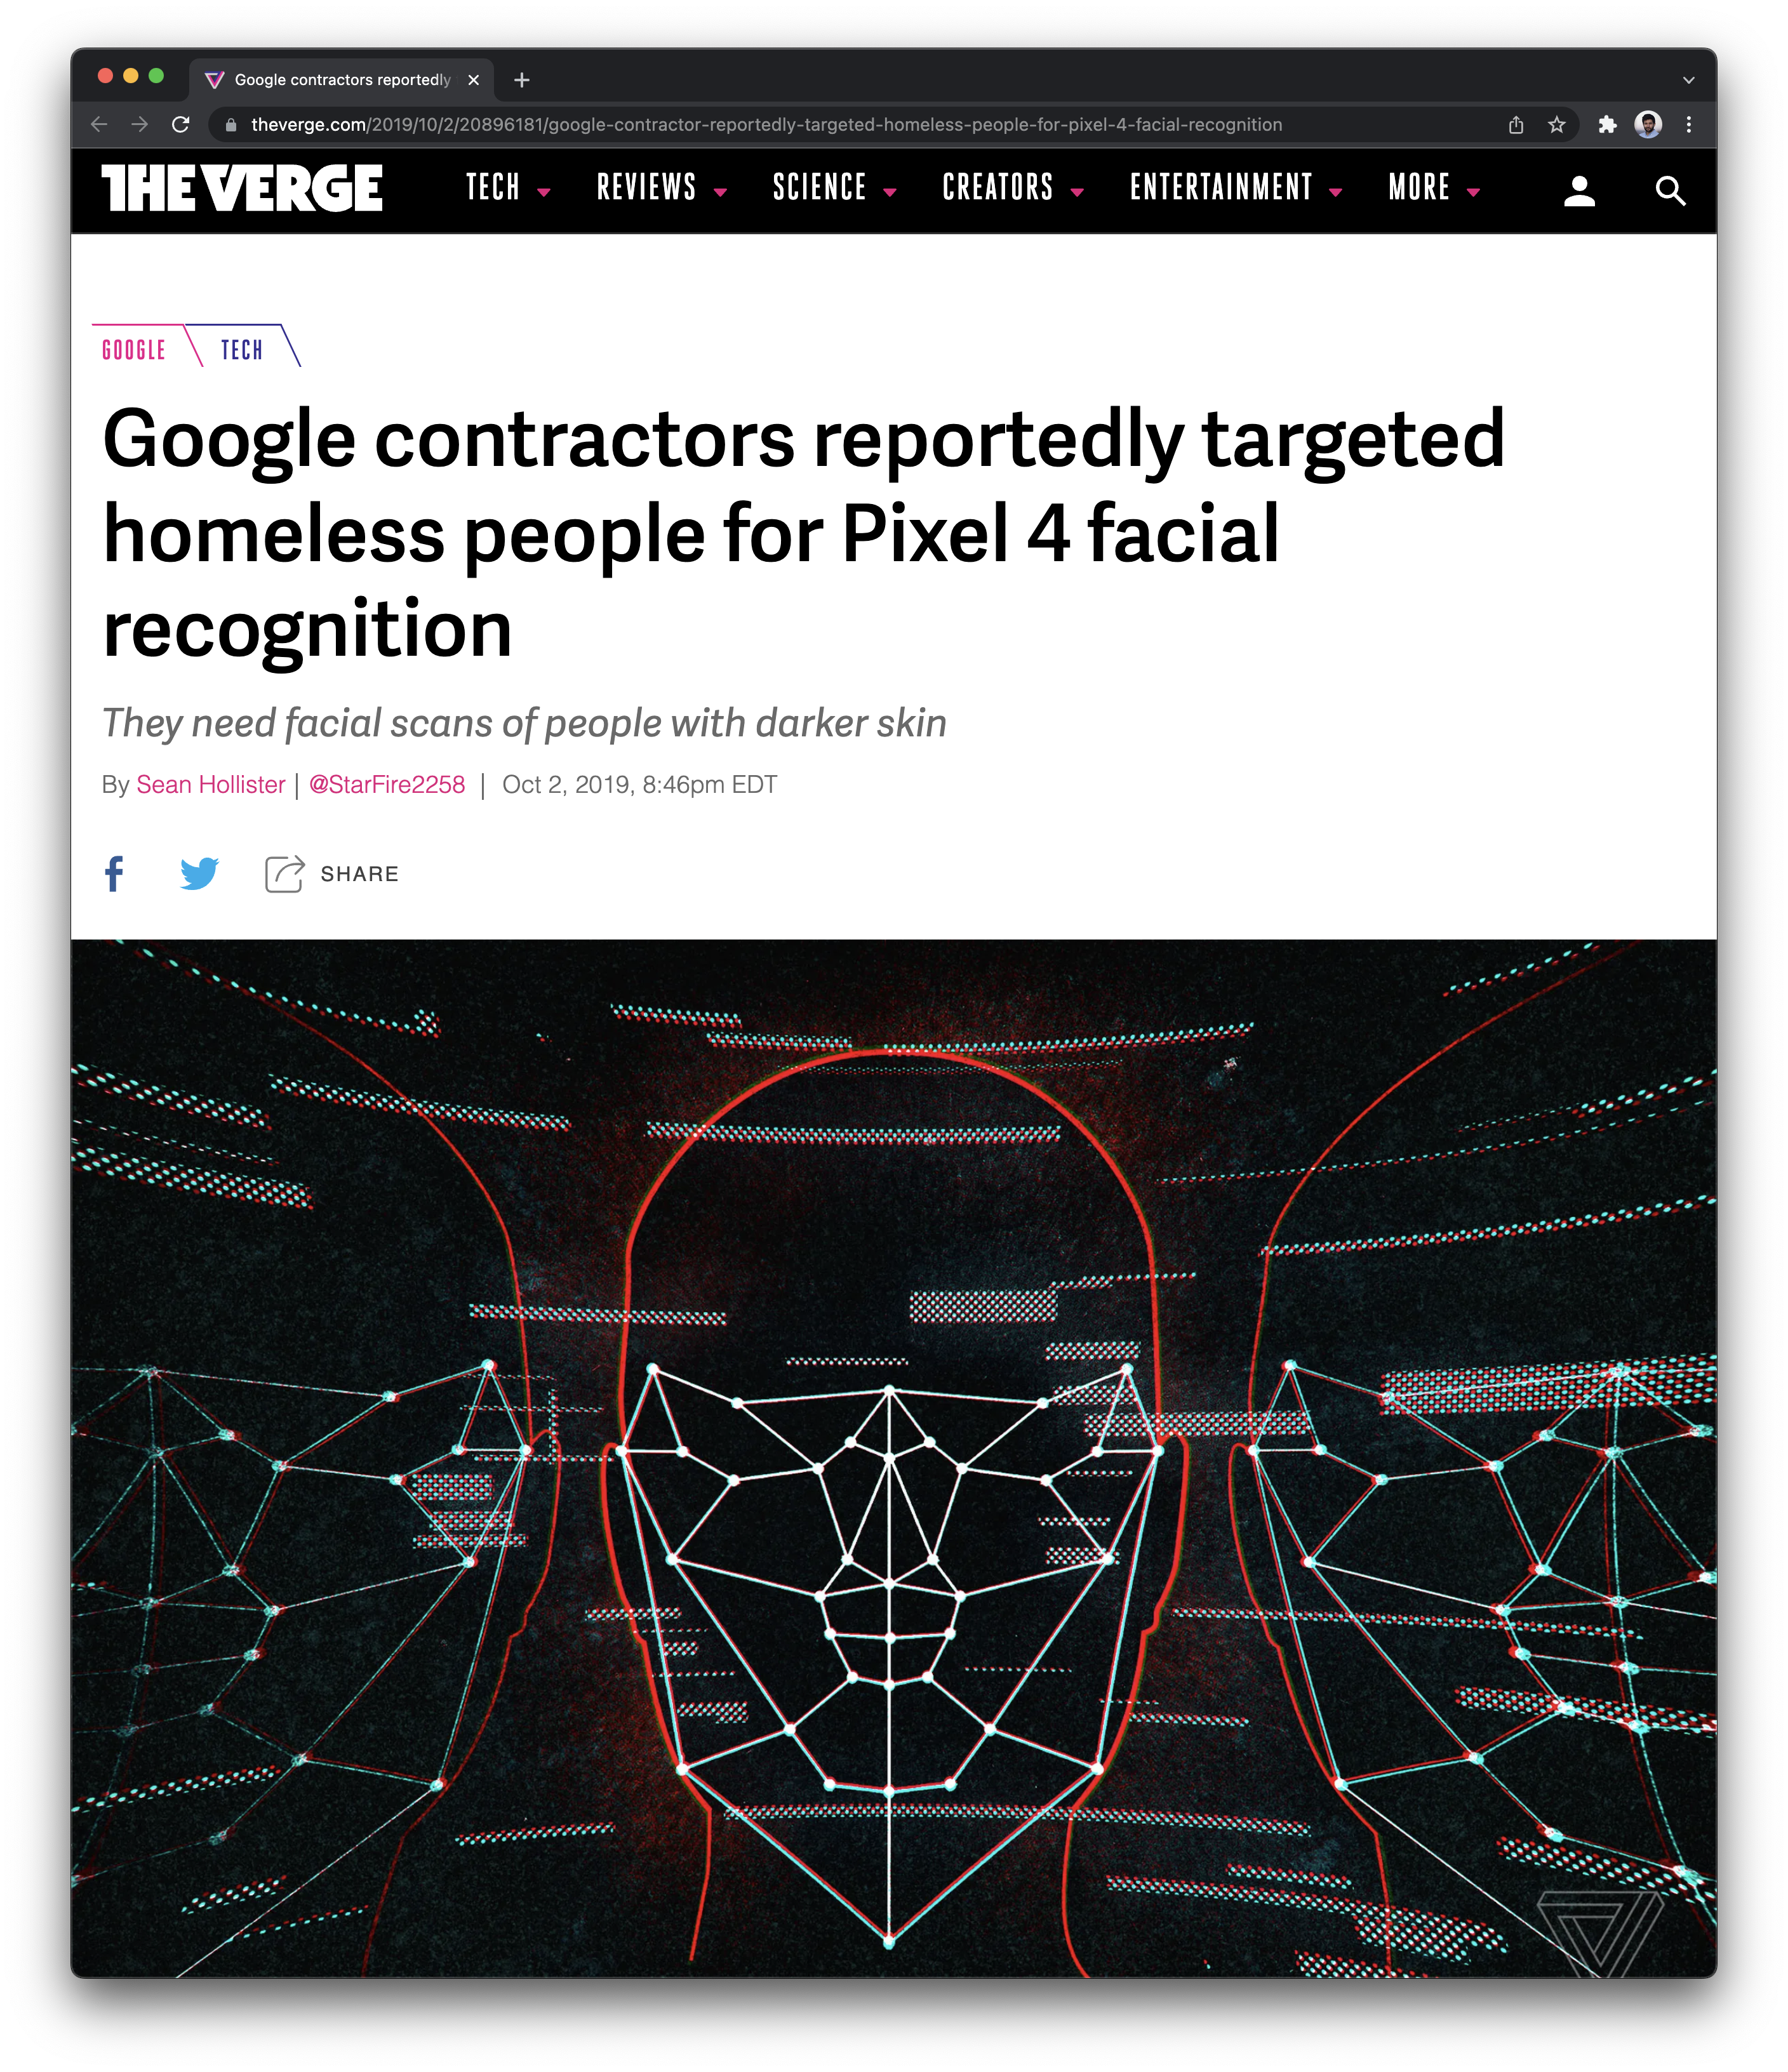
\includegraphics[width=\textwidth]{figures/consent/google.png}}
\only<5>{\includegraphics[width=\textwidth]{figures/consent/GDPR.png}}
\only<6>{\includegraphics[width=\textwidth]{figures/consent/CCPA.png}}
\end{column}
\end{columns}

\end{frame}

\begin{frame}[plain]

\centering

\visible<+->{{\LARGE\scshape legal $\centernot\implies$ ethical}}

\visible<+->{\dots but\dots}

\visible<+->{the \textbf<.>{law} can be\\\textbf<+>{narrowly} informative}

\end{frame}


% \begin{frame}[standout]
% what questions should you be asking?
% \end{frame}


\begin{frame}[plain]

{\scshape\small
\centering
\begin{columns}
\begin{column}{0.3\textwidth}
\centering

\visible<+->{repugnance}

\visible<+->{potential for harm}

\visible<+->{\textbf<+->{misleading}}

\visible<+->{false pretenses}


\end{column}
\begin{column}{0.3\textwidth}
\centering

\visible<+->{exploitation}

\visible<+->{firing personnel}


\visible<+->{CYA}

\visible<+->{speed of tech}
\end{column}
\begin{column}{0.3\textwidth}
\centering

\visible<+->{intent vs outcome}

\visible<+->{incentives}

\visible<+->{\textbf<+->{vulnerability}}

\visible<+->{misuse}

\visible<+->{apparent plan (or lack of?)}

\end{column}
\end{columns}


\visible<+->{``Shouldn't regulators have gotten involved?''}

\visible<+->{``\dots the laws we have today are from to 1970's?''}


}
\end{frame}

\begin{frame}{Philosophical frameworks}

{\scshape\onslide<+>{}

\onslide<+->{Consequentialism}{\small\visible<.->{\onslide<.>{\hfill evaluate by outcomes}}}

\onslide<+->{Deontology}{\small\visible<.->{\onslide<.>{\hfill evaluate by rules}}}

\onslide<+->{Virtue Ethics}{\small\visible<.->{\onslide<.>{\hfill evaluate by aspirational virtues}}}

}
\end{frame}


\begin{frame}{historical contextualization}
\centering

\only<1>{\begin{columns}
\begin{column}{0.6\textwidth}
\only<1>{Henrietta Lacks}
\only<2>{Henrietta Lacks}
\end{column}
\begin{column}{0.4\textwidth}
\only<2>{\includegraphics[width=\textwidth]{figures/wiki/lacks.jpeg}}
\only<1>{\includegraphics[width=\textwidth]{figures/wiki/lacks.jpeg}}
\end{column}
\end{columns}}

{\scshape
\only<2->{human dignity and autonomy}

\only<3->{informed consent}
}
\end{frame}







\begin{frame}{speculative design}
\centering
\includegraphics[height=0.9\textheight]{figures/clipart/speculative_design.png}
\end{frame}



\begin{frame}{some ``provocations''}
\end{frame}


\begin{frame}[plain]
\centering

a quick caveat about ``provocations''

\end{frame}

\begin{frame}{some ``provocations''}
\vspace{2em}
{\footnotesize
\begin{columns}
\begin{column}{0.5\textwidth}
{What are the risks of allowing the private sector to gather so much sensitive data?}

\vspace{1em}

{Does anyone else feel uncomfortable about statements about suicide prevention efforts using phrases like ``piloting a tailored solution'' and ``evaluating data trends?''}

\vspace{1em}

{What would it look like if all of the [face] scans of POC came from \emph{marginalized} populations?}
\end{column}
\begin{column}{0.5\textwidth}
{When do we know that an issue having to do with privacy and surveillance has been adequately addressed?}

\vspace{1em}

{At what point do the negatives of a technology that gathers data outweigh the positives? Likewise, when do the positives outweigh the negatives?}
% \end{column}
% \begin{column}{0.33\textwidth}


\end{column}
\end{columns}}

\end{frame}


% {what are some examples of how data science uses hypotheticals to understand and predict ethical issues? what about using models as a more concrete way to evaluate if a particular kind of data collection will cause harm?}
%

\end{document}
